\chapter{Results}
\label{cha:results}

This chapter covers the results from the 2011 Kukui Cup challenge, and how those results address my research questions:

\begin{enumerate}
	\item To what extent did residents participate in the challenge?
	\item How did energy literacy change after the challenge?
	\item How did energy use change during the challenge?
	\item How did energy use change after the challenge?
	\item What is the relationship between energy literacy and energy usage?
	\item How effective were the actions available via the website?
	\item How appropriate were the point values assigned to actions?
	\item How important was lounge-level near-realtime feedback?
\end{enumerate}

I begin by examining participation in the challenge, which is supported primarily through log data from the website itself (RQ\#1). Second, I turn to an examination of energy literacy using the results from the pre- and post-challenge energy literacy questionnaire (RQ\#2 and \#5). Next, I cover the energy use before, during, and after the challenge (RQ\#3 and \#4), including a discussion on baselines. The following sections address the remaining research questions (RQ \#6, \#7, and \#8), and some additional results unanticipated by the research questions.


\section{Website Adoption}

Research Question 1 is ``to what extent did residents participate in the challenge?''. I address this question using data collected from the challenge website logs. First, I examine individual participation as measured by points earned via the challenge website. Next, I review the number of actions completed by players through the website. Finally, I cover the participation of players on a lounge by lounge basis.

\subsection{Individual Participation}
\label{sec:individual-participation}

According to a roster provided by Student Housing (which we used to populate user accounts for the challenge website), there were 1072 residents in the Hale Aloha towers during the challenge, including the 40 Resident Advisors. This number is approximate, because there were some errors in the roster, and residents sometimes move in or out of the residence halls. However, these changes are small and usually move-outs are balanced by move-ins.

According to the challenge website logs, 18 users logged into the website, but did not complete the first-login process.

Of the 1072 potential participants, 401 scored 25 points or more in the challenge (the threshold established in \autoref{sec:participation}), for a participation rate of 37\%.

As mentioned in \autoref{sec:referral-bonus}, in Round 2 we instituted a referral bonus. 38.3\% (159) of users logging into the challenge website for the first time entered in a referring email address. Of those referred users, 93\% (148) went on to earn at least 30 points and earn the bonus. Given that the bonus was introduced in Round 2, this figure represents a significant use of the bonus.

\autoref{fig:referrals-per-referer} shows the frequency distribution of the participants making the referral. All the referrals were made by only 20 participants, and the top two referrers accounted for 66\% of all referrals made.

\begin{figure}[htbp]
%% Chart from user_experience_analysis-1-rsb.xlsx!Referrals
	\centering
	\includegraphics[scale=0.75]{referrals-per-referer-histogram2}
	\caption[Histogram of number of referrals versus the number players]{Histogram of number of referrals versus the number players who made that number of referrals.}
	\label{fig:referrals-per-referer}
\end{figure}

One reason for the concentration of referrals by two participants was due to the challenge endgame. The overall point totals for the top two participants were very close as the Overall Round drew to a close. Having earned the vast majority of the points available through the Smart Grid Game, they seized on the referral bonus as an open-ended way to earn additional points. The two players attempted to sign up as many new participants as they could. On the final day, the overall winner reported that they used the participation scoreboard to determine which lounge had the lowest overall participation, and went door-to-door asking residents to log onto the challenge website and complete one activity to help the referrer win the challenge! On the final day of the challenge, there were 68 first-time users (67 matching the 25 point participation threshold discussed in \autoref{sec:participation}), and all of entered a referring email address, showing the impact of this referral bonus endgame.

While these final-day participants may have learned more about energy through their participation in online activities, by participating for less than a day they probably did not contribute significantly to energy conservation efforts in their lounge. Without this final day surge, the participation rate would be 31\%. \autoref{fig:participants-over-time} shows how the number of new and total participants varied over the challenge period.

\begin{figure}[htbp]
%% Chart from "Points over time.xlsx"!"Players over time"
	\centering
	\includegraphics[scale=0.7]{participants-over-time2}
	\caption{Number of new and total participants per day of challenge}
	\label{fig:participants-over-time}
\end{figure}


%\subsection{Time Spent on Challenge Website}


\subsection{Player Action Submissions}

Players earn points by completing actions through the challenge website. During the challenge, players completed a total of 4,641 actions. \autoref{fig:actions-completed} shows a histogram of the number of actions completed versus the number of users that completed that number. While there are clearly many players that only completed one or two actions (some of them from the referral bonus surge), there is a long tail of players that completed many actions in the game.

\begin{figure}[htbp]
%% Chart from user_experience_analysis-1-rsb.xlsx!Smart Grid
	\centering
	\includegraphics[width=\textwidth]{number-actions-completed}
	\caption{Number of players that completed a certain number of actions.}
	\label{fig:actions-completed}
\end{figure}


\subsection{Lounge Participation}
\label{sec:lounge-participation}

Using the same 25 point participation threshold, I can compute the aggregate participation rate for each lounge. \autoref{tab:lounge-participation} shows the participation rate and total score for each lounge at the end of each of the three rounds of the challenge. The lounges that won the point challenge for each round are shown in bold. This table shows the significant disparities in participation between lounges, with three lounges participating at 15\% or less, and the with the best lounge participating at 74\%.

%% Using \multicolumn to make spanning columns & to remove border from 1st cell
\begin{table}[htbp]
%% Data from "Points over time.xlsx"!"Lounge participation"
	\centering
	\caption[Score and participation per lounge at the end of each round]{Score and participation per lounge at the end of each round, bold entries indicate round winners. Note that the Round 2 score started from zero (reset), not from the Round 1 total, but participation is cumulative.}
	\label{tab:lounge-participation}
	\vskip 1em
	\begin{tabular}{ l | c | r | c | r | c | r |}
		\cline{2-7}
		 & \multicolumn{2}{c|}{Round 1} & \multicolumn{2}{c|}{Round 2} & \multicolumn{2}{c|}{Overall Round} \\ \hline
		\multicolumn{1}{|l|}{Lounge} & Participation & Score & Participation & Score & Participation & Score \\ \hline \hline
		\multicolumn{1}{|l|}{Ilima-A} & 37\% & 5152 & 69\% & \textbf{3893} & 74\% & \textbf{12840} \\ \hline
		\multicolumn{1}{|l|}{Ilima-B} & 19\% & 755 & 26\% & 725 & 35\% & 2248 \\ \hline
		\multicolumn{1}{|l|}{Ilima-C} & 11\% & 754 & 13\% & 395 & 15\% & 1472 \\ \hline
		\multicolumn{1}{|l|}{Ilima-D} & 13\% & 264 & 22\% & 762 & 26\% & 1469 \\ \hline
		\multicolumn{1}{|l|}{Ilima-E} & 11\% & 406 & 11\% & 275 & 13\% & 1251 \\ \hline
		\multicolumn{1}{|l|}{Lehua-A} & 7\% & 373 & 15\% & 526 & 15\% & 1493 \\ \hline
		\multicolumn{1}{|l|}{Lehua-B} & 19\% & 1831 & 24\% & 1377 & 44\% & 5214 \\ \hline
		\multicolumn{1}{|l|}{Lehua-C} & 13\% & 1140 & 24\% & 1596 & 31\% & 3868 \\ \hline
		\multicolumn{1}{|l|}{Lehua-D} & 33\% & 4898 & 37\% & 1957 & 44\% & 8963 \\ \hline
		\multicolumn{1}{|l|}{Lehua-E} & 43\% & \textbf{5288} & 44\% & 1549 & 52\% & 7702 \\ \hline
		\multicolumn{1}{|l|}{Lokelani-A} & 17\% & 389 & 56\% & 2630 & 67\% & 5087 \\ \hline
		\multicolumn{1}{|l|}{Lokelani-B} & 13\% & 455 & 20\% & 168 & 30\% & 1219 \\ \hline
		\multicolumn{1}{|l|}{Lokelani-C} & 24\% & 1344 & 31\% & 598 & 35\% & 2391 \\ \hline
		\multicolumn{1}{|l|}{Lokelani-D} & 11\% & 335 & 15\% & 637 & 26\% & 1585 \\ \hline
		\multicolumn{1}{|l|}{Lokelani-E} & 15\% & 1989 & 19\% & 849 & 22\% & 3858 \\ \hline
		\multicolumn{1}{|l|}{Mokihana-A} & 15\% & 745 & 37\% & 1820 & 54\% & 4436 \\ \hline
		\multicolumn{1}{|l|}{Mokihana-B} & 13\% & 994 & 19\% & 837 & 31\% & 3427 \\ \hline
		\multicolumn{1}{|l|}{Mokihana-C} & 6\% & 328 & 17\% & 498 & 37\% & 1501 \\ \hline
		\multicolumn{1}{|l|}{Mokihana-D} & 7\% & 574 & 19\% & 1270 & 37\% & 4351 \\ \hline
		\multicolumn{1}{|l|}{Mokihana-E} & 24\% & 2104 & 39\% & 3318 & 54\% & 8837 \\ \hline
	\end{tabular}
\end{table}

As discussed in \autoref{sec:individual-participation}, the final day surge of participants inflates the participation rate of lounges. \autoref{tab:lounge-minus-endgame} shows the final participation rates with and without the final day surge, while \autoref{fig:lounge-participation} shows a plot ordered by participation rate. The participation rate without the final surge is more appropriate when the participation is being compared to other data, such as energy use, which would not have been significantly impacted by participants who joined on the final day of the challenge.

\begin{table}[htbp]
%% Data from "Points over time.xlsx"!"Lounge charts"
	\centering
	\caption{Overall Lounge participation with and without final day surge}
	\label{tab:lounge-minus-endgame}
	\vskip 1em
	\begin{tabular}{| l | c | c |}
		\hline
		Lounge & Overall participation & Minus final day \\ \hline
		Ilima-A & 74\% & 69\% \\ \hline
		Ilima-B & 35\% & 26\% \\ \hline
		Ilima-C & 15\% & 13\% \\ \hline
		Ilima-D & 26\% & 22\% \\ \hline
		Ilima-E & 13\% & 11\% \\ \hline
		Lehua-A & 15\% & 15\% \\ \hline
		Lehua-B & 44\% & 31\% \\ \hline
		Lehua-C & 31\% & 26\% \\ \hline
		Lehua-D & 44\% & 39\% \\ \hline
		Lehua-E & 52\% & 50\% \\ \hline
		Lokelani-A & 67\% & 63\% \\ \hline
		Lokelani-B & 30\% & 22\% \\ \hline
		Lokelani-C & 35\% & 33\% \\ \hline
		Lokelani-D & 26\% & 19\% \\ \hline
		Lokelani-E & 22\% & 19\% \\ \hline
		Mokihana-A & 54\% & 54\% \\ \hline
		Mokihana-B & 31\% & 24\% \\ \hline
		Mokihana-C & 37\% & 24\% \\ \hline
		Mokihana-D & 37\% & 20\% \\ \hline
		Mokihana-E & 54\% & 39\% \\ \hline
	\end{tabular}
\end{table}

\begin{figure}[htbp]
%% Chart from "Points over time.xlsx"!"Lounge charts"
	\centering
	\includegraphics[width=\textwidth]{lounge-participation2}
	\caption{Plot of overall Lounge participation with and without final day surge}
	\label{fig:lounge-participation}
\end{figure}


\subsection{Discussion}

Based on the data presented here, 37\% of residents participated in the challenge by earning 25 points or more. Most energy competitions are unable to provide any data on participation rates, because they don't have any easy way to measure participation. While most energy competitions have a website, the website is not necessarily essential for participation, unlike the Kukui Cup; therefore, measurement of website use is not a good measure of participation for other competitions.

The Oberlin dorm energy competition did have a central website for energy feedback. For their 2005 competition, they report 4,082 ``hits'', and determined that 46\% of dormitory residents viewed the website based on IP address logs~\cite{petersen-dorm-energy-reduction}. However the Oberlin system did not ask users to log in or interact with the site in any way, so that reflects a less in-depth interaction compared to participation in the Kukui Cup website. The participation rate in the 2011 Kukui Cup appears comparable to the Oberlin results, and the evidence of participation is much clearer in the Kukui Cup due to the unifying website.

Participation over the challenge at the lounge level varied significantly between lounges, ranging from 69\% to 11\% (without final day surge). This range reflects lounges with high participation and high scores, such as Lehua E in Round 1), as well as lounges with a smaller number of participants each earning higher scores, such as Lokelani E in Round 1. Based on interactions with players at award events, it was clear that some lounges had highly active players who were able to rally other residents in their lounge to participate, while other highly active players were unable or unwilling to get other loungemates to participate.

In answer to research question \#1, based on the results shown here, many residents chose to participate in the Kukui Cup. Obviously, participation was essential to the success of the Kukui Cup.


\section{Energy Literacy Questionnaire}
\label{sec:energy-lit-results}

As discussed in \autoref{sec:energy-literacy-exp}, I administered an online energy literacy questionnaire to a set of residents in Hale Aloha twice: once before the challenge, and once after the challenge. This section covers the results from those questionnaires. The full text of the questions can be found in \autoref{app:energy-literacy}.

\subsection{Questionnaire Responses}

Since each subject was to be compensated for participating in the questionnaire, and I did not know beforehand how many potential subjects would actually participate, I sent the questionnaire invitation in two waves. The first wave of 74 email invitations was sent on October 5, 2011, and a second wave of 107 invitations was sent on October 10. 68 questionnaires were completed, which is a response rate of 38\%. There were 5 partial responses, but in each case the subjects abandoned the survey before submitting any data other than the informed consent page, I have not included those subjects in the following analyses.

After the challenge was complete, I sent the same questionnaire to all the individuals that had participated in the pre-challenge questionnaire. There were 51 complete responses, and 2 responses that stopped after filling out the consent form. Since the questionnaire was administered before the challenge began, I could not tell in advance how many subjects would go on to participate in the challenge. As discussed in \autoref{sec:participation}, I call subjects participants if they earned 25 points in the challenge. \autoref{tab:questionnaire-responses} shows the number of questionnaire responses from participants and non-participants, and those that completed both questionnaires. 48 subjects completed both the pre-challenge and post-challenge questionnaires, evenly split between participants and non-participants. None of the 48 subjects that completed both questionnaires were RAs, so all subjects were first-year students. One subject moved out of Hale Aloha before the challenge started, and another moved out during the challenge. Neither of the two logged into the challenge website.

\begin{table}[htbp]
%% Data from SurveyExport.xlsx!Participation
	\centering
	\caption{Number of completed pre- and post-challenge questionnaires.}
	\label{tab:questionnaire-responses}
	\vskip 1em
	\begin{tabular}{| l | c | c | c |}
		\hline
		Subject type & Pre-challenge & Post-challenge & Completed both \tabularnewline \hline \hline
		Non-challenge participants & 36 & 27 & 24 \tabularnewline \hline
		Challenge participants & 32 & 24 & 24 \tabularnewline \hline \hline
		Total & 68 & 51 & 48 \tabularnewline \hline
	\end{tabular}
\end{table}

The relatively small number of subjects that completed both pre- and post-challenge questionnaires were spread over the 20 lounges. \autoref{tab:subject-lounges} shows the distribution across the lounges. Note that the one subject that moved out before the challenge started was not listed in the roster we received from Student Housing, so their lounge is unknown.

\begin{table}[htbp]
%% Data from "SurveyExport.xlsx"!"subject lounges"
	\centering
	\caption{Distribution of questionnaire participants across lounges.}
	\label{tab:subject-lounges}
	\vskip 1em
	\begin{tabular}{| l | c |}
		\hline
		Lounge & Number of subjects \\ \hline
		Ilima-A & 1 \\ \hline
		Ilima-B & 6 \\ \hline
		Ilima-C & 2 \\ \hline
		Ilima-D & 1 \\ \hline
		Ilima-E & 1 \\ \hline
		Lehua-A & 2 \\ \hline
		Lehua-B & 3 \\ \hline
		Lehua-C & 2 \\ \hline
		Lehua-D & 2 \\ \hline
		Lehua-E & 1 \\ \hline
		Lokelani-A & 1 \\ \hline
		Lokelani-B & 0 \\ \hline
		Lokelani-C & 3 \\ \hline
		Lokelani-D & 1 \\ \hline
		Lokelani-E & 4 \\ \hline
		Mokihana-A & 4 \\ \hline
		Mokihana-B & 3 \\ \hline
		Mokihana-C & 3 \\ \hline
		Mokihana-D & 3 \\ \hline
		Mokihana-E & 4 \\ \hline
		Unknown & 1 \\ \hline
	\end{tabular}
\end{table}


\subsection{Energy Knowledge}

The energy knowledge section of the questionnaire consisted of 19 factual questions about energy, with a specific emphasis on \Hawaii energy issues. \autoref{tab:knowledge-descriptives} shows the average number of questions answered correctly for participants and non-participants in the pre- and post-challenge questionnaires. Non-participants showed no change in the number of questions answered correctly after the challenge, while participants improved by 18.8\%. \autoref{fig:knowledge-anova} is a plot of the results. Using ANOVA, there was a significant interaction between participation and differences between pre- and post-challenge scores, \(F(1, 46) = 3.84\), \(p = 0.056\), MSE \(= 3.52\). Challenge participants scores improved, and non-challenge-participants energy knowledge scores were unchanged. Therefore, this result supports the hypothesis that participating in the Kukui Cup increases the energy literacy of participants.


\begin{table}[htbp]
%% Data from Survey-analysis-results.xlsx!Knowledge & SPSS results
	\centering
	\caption[Energy knowledge before and after challenge]{Average number of energy knowledge questions correct for participants and non-participants before and after the challenge}
	\label{tab:knowledge-descriptives}
	\vskip 1em
	\begin{tabular}{ l | c | c | c | c | c }
		\cline{2-5}
		& \multicolumn{2}{c |}{Pre-challenge} & \multicolumn{2}{c|}{Post-challenge} & \\ \hline
		\multicolumn{1}{|l|}{Subject type} & Mean & Std. Deviation & Mean & Std. Deviation & \multicolumn{1}{c|}{\% Change} \tabularnewline \hline \hline
		\multicolumn{1}{|l|}{Non-challenge participants} & 7.46 & 2.377 & 7.37 & 2.570 & \multicolumn{1}{c|}{-1.2\%} \tabularnewline \hline
		\multicolumn{1}{|l|}{Challenge participants} & 7.54 & 1.837 & 8.96 & 3.290 & \multicolumn{1}{c|}{18.8\%} \tabularnewline \hline
	\end{tabular}
\end{table}

\begin{figure}[htbp]
%% Data from Survey-analysis-results.xlsx!Knowledge & SPSS results
	\centering
	\includegraphics[width=0.6\textwidth]{knowledge-anova}
	\caption[Plot of energy knowledge before and after challenge]{Plot of average number of energy knowledge questions correct for participants and non-participants before and after the challenge}
	\label{fig:knowledge-anova}
\end{figure}

\autoref{fig:knowledge-questions} shows the percentage of subjects that correctly answered each of the 19 questions in the energy literacy section, from most correct to least correct. The full text of each question can be found in \autoref{sec:knowledge-items}.

\begin{figure}[htbp]
%% Data from Survey-analysis-results.xlsx!Knowledge & SPSS results
	\centering
	\includegraphics[width=\textwidth]{knowledge-questions}
	\caption[Plot of energy knowledge before and after challenge]{Percentage of correct answers for each energy knowledge question}
	\label{fig:knowledge-questions}
\end{figure}


\subsection{Energy Attitudes}

The energy attitudes section of the questionnaire was taken from the affective subscale of the energy literacy questionnaire developed by DeWaters and Powers~\cite{DeWaters2011}. There are 18 statements in the attitudes section using a five-point Likert scale from 1 for ``strongly agree'' to 5 for ``strongly disagree'', where strongly agree was the most preferred response for positive energy attitudes. \autoref{tab:attitude-descriptives} shows the average rating value across all 18 statements for participants and non-participants in the pre- and post-challenge questionnaires. \autoref{fig:attitude-anova} is a plot of the results.

\begin{table}[htbp]
%% Data from Survey-analysis-results.xlsx!Attitude & SPSS results
	\centering
	\caption[Energy attitudes before and after challenge]{Average energy attitude scores for participants and non-participants before and after the challenge}
	\label{tab:attitude-descriptives}
	\vskip 1em
	\begin{tabular}{ l | c | c | c | c | c }
		\cline{2-5}
		& \multicolumn{2}{c |}{Pre-challenge} & \multicolumn{2}{c|}{Post-challenge} & \\ \hline
		\multicolumn{1}{|l|}{Subject type} & Mean & Std. Deviation & Mean & Std. Deviation & \multicolumn{1}{c|}{\% Improved} \tabularnewline \hline \hline
		\multicolumn{1}{|l|}{Non-challenge participants} & 2.23 & 0.438 & 2.11 & 0.561 & \multicolumn{1}{c|}{5.5\%} \tabularnewline \hline
		\multicolumn{1}{|l|}{Challenge participants} & 2.11 & 0.428 & 2.13 & 0.719 & \multicolumn{1}{c|}{-0.8\%} \tabularnewline \hline
	\end{tabular}
\end{table}

\begin{figure}[htbp]
%% Chart from Survey-analysis-results.xlsx!Attitude & SPSS results
	\centering
	\includegraphics[width=0.8\textwidth]{attitude-anova}
	\caption[Plot of energy attitudes before and after challenge]{Plot of average energy attitude scores for participants and non-participants before and after the challenge}
	\label{fig:attitude-anova}
\end{figure}

Non-participants showed a small improvement in their attitude score in the post-challenge questionnaire, while participants' scores decreased slightly, but these results were not statistically significant. These results indicate that the 2011 Kukui Cup did not change the attitude of participants towards energy conservation and renewable energy. It may be that the three week challenge length was not long enough to change attitudes, or perhaps the challenge's focus on direct energy conservation actions took away from potential changes in attitude.

Because the attitude section of the questionnaire is a slightly modified version of the DeWaters and Powers attitude subscale, it is worth comparing their results with high school students to the results from my subjects. DeWaters and Powers normalized their values to percentages (where 100\% would be the most preferred answer to all questions), so for comparison purposes I have done the same normalization.

\begin{table}[htbp]
%% Chart from Survey-analysis-results.xlsx!Attitude
	\centering
	\caption{Comparison of attitude scores between Kukui Cup and DeWaters and Powers results.}
	\label{tab:attitude-comparison}
	\vskip 1em
	\begin{tabular}{| l | c | c | c |}
		\hline
		Subject type & Pre-challenge & Post-challenge & New York State \tabularnewline \hline \hline
		Non-challenge participants & 69.3\% & 72.4\% & \tabularnewline \hline
		Challenge participants & 72.2\% & 71.8\% & \tabularnewline \hline
		Middle School & & & 73.0\% \tabularnewline \hline
		High School & & & 73.9\% \tabularnewline \hline \hline
	\end{tabular}
\end{table}

\autoref{tab:attitude-comparison} shows the comparison. The New York State students very similar attitude scores compared to the Hale Aloha subjects. Since the Hale Aloha subjects were all in their first semester of college, their attitudes could be expected to be similar to that of high school students.


\subsection{Reported Energy Behaviors}

The energy behavior section of the questionnaire consisted of 17 statements about energy use behaviors inspired by the energy literacy instrument developed by DeWaters and Powers~\cite{DeWaters2011}. Each statement was rated on a scale from 1 for ``always or almost always'' to 5 for ``never or hardly ever'', where always or almost always was the most preferred response for positive energy behaviors. \autoref{tab:behavior-descriptives} shows the average rating value across all 17 statements for participants and non-participants in the pre and post-challenge questionnaires. Non-participants showed a small improvement in their behavior score in the post-challenge questionnaire, with participants showing a slightly larger improvement. \autoref{fig:behavior-anova} is a plot of the results.

\begin{table}[htbp]
	\centering
	\caption[Reported energy behaviors before and after challenge]{Average self-reported energy behavior scores for participants and non-participants before and after the challenge}
	\label{tab:behavior-descriptives}
	\vskip 1em
	\begin{tabular}{ l | c | c | c | c | c }
		\cline{2-5}
		& \multicolumn{2}{c |}{Pre-challenge} & \multicolumn{2}{c|}{Post-challenge} & \\ \hline
		\multicolumn{1}{|l|}{Subject type} & Mean & Std. Deviation & Mean & Std. Deviation & \multicolumn{1}{c|}{\% Improved} \tabularnewline \hline \hline
		\multicolumn{1}{|l|}{Non-challenge participants} & 2.56 & 0.510 & 2.52 & 0.596 & \multicolumn{1}{c|}{1.7\%} \tabularnewline \hline
		\multicolumn{1}{|l|}{Challenge participants} & 2.52 & 0.443 & 2.35 & 0.339 & \multicolumn{1}{c|}{6.6\%} \tabularnewline \hline
	\end{tabular}
\end{table}

\begin{figure}[htbp]
	\centering
	\includegraphics[width=0.8\textwidth]{behavior-anova}
	\caption[Plot of energy behavior before and after challenge]{Plot of average self-reported energy behavior scores for participants and non-participants before and after the challenge}
	\label{fig:behavior-anova}
\end{figure}

Using ANOVA, I found there was a significant difference between pre and post-challenge scores, \(F(1, 46) = 4.09\), \(p = 0.049\), MSE \(= 2.94\), but interaction between participation and pre and post-challenge scores was not significant. Since the self-reports of behavior changes took place for both participants and non-participants, these changes provide the interesting possibility of \emph{passive participants} who made changes in their behavior due to the challenge, but did not participate in the challenge (based on my definition participation: earning 25 points). It is not hard to imagine that non-participants might find themselves changing their behaviors due to requests from roommates who are participating, or new social norms developing as a result of participants' behavior, because most of the targeted behaviors are public and some involve shared resources (such as the overhead lighting in residents' rooms). Future iterations of the Kukui Cup could encourage these changes in behavior even among non-participants through additional activities that target non-participants (``get your non-participating roommate to take the stairs'') or additional marketing materials designed around establishing new social norms as described in \autoref{sec:norms}.


\subsection{Group Identification}
\label{sec:group-id}

I used the Arrow-Carini Group Identification Scale 2.0~\cite{Henry1999} for the group identification section of the questionnaire. It consists of 12 statements in three subscales: affective, behavioral, and cognitive. Subjects were asked to respond to each one on a seven-point Likert scale from 1 for ``strongly disagree'' to 7 for ``strongly agree'', where strongly agree was the response that reflected the most group identification. The group specified in the statements was the lounge that subjects belong to, since lounges represent the teams in the Kukui Cup. \autoref{tab:group-id-descriptives} shows the average scale value for participants and non-participants in the pre and post-challenge questionnaires, while \autoref{fig:group-id-anova} shows a plot of the results.

\begin{table}[htbp]
	\centering
	\caption[Group identity score before and after challenge]{Average group identification scores for participants and non-participants before and after the challenge}
	\label{tab:group-id-descriptives}
	\vskip 1em
	\begin{tabular}{ l | c | c | c | c | c }
		\cline{2-5}
		& \multicolumn{2}{c |}{Pre-challenge} & \multicolumn{2}{c|}{Post-challenge} & \\ \hline
		\multicolumn{1}{|l|}{Subject type} & Mean & Std. Deviation & Mean & Std. Deviation & \multicolumn{1}{c|}{\% Change} \tabularnewline \hline \hline
		\multicolumn{1}{|l|}{Non-challenge participants} & 4.10 & 0.869 & 4.14 & 0.872 & \multicolumn{1}{c|}{1.0\%} \tabularnewline \hline
		\multicolumn{1}{|l|}{Challenge participants} & 4.13 & 0.823 & 3.79 & 0.963 & \multicolumn{1}{c|}{-8.0\%} \tabularnewline \hline
	\end{tabular}
\end{table}

\begin{figure}[htbp]
	\centering
	\includegraphics[width=0.8\textwidth]{group-id-anova}
	\caption[Plot of group identification before and after challenge]{Plot of average group identification scores for participants and non-participants before and after the challenge}
	\label{fig:group-id-anova}
\end{figure}

Both participants and non-participants were neutral towards their lounge. Participants showed a decline of 8\% in their group identification with the lounge, while non-participants were mostly unchanged. These results were not statistically significant, but they provide interesting possibilities to be investigated further. While I had hypothesized that the Kukui Cup experience would increase participants' identification with the lounge, it may be that participants started to identify with other Kukui Cup participants rather than fellow loungemates. Another possible scenario could be that dedicated participants who are trying to reduce their lounge's energy use might find themselves alienated from their loungemates who are not making an effort to conserve energy.

In developing the scale, Henry et al. compared subjects who completed the scale once for a group they belonged to that they considered highly important to them, and again for a group they did not consider important. Henry et al. found the average score for important groups was 5.93, while for the unimportant groups it was 3.89, which is close to the averages I found for lounge identification. Therefore, it appears that subjects do not consider the lounge they belong to as an important group.

It is worth noting that two subjects indicated in the questionnaire feedback that they did not know what a lounge was (see \autoref{questionnaire-feedback}), and all the group identification statements referred to the subjects' lounge. It is possible that other subjects also did not understand the lounge grouping, which could also explain the neutral ranking and lack of significant change after the challenge.


\subsection{Connectedness to Nature}

For the connectedness to nature section of the questionnaire, I used the CNS scale developed by Mayer and Frantz~\cite{MayerFrantz2004}. It consists of 14 statements regarding the relationship between humans and nature. Subjects were asked to respond to each statement on a five-point Likert scale from 1 for ``strongly disagree'' to 5 for ``strongly agree'', where strongly agree was the response that reflected the most connectedness to nature.  \autoref{tab:cns-descriptives} shows the average scale value for participants and non-participants in the pre- and post-challenge questionnaires, while \autoref{fig:cns-anova} shows a plot of the results.

\begin{table}[htbp]
	\centering
	\caption[CNS score before and after challenge]{Average connectedness to nature scores for participants and non-participants before and after the challenge}
	\label{tab:cns-descriptives}
	\vskip 1em
	\begin{tabular}{ l | c | c | c | c | c }
		\cline{2-5}
		& \multicolumn{2}{c |}{Pre-challenge} & \multicolumn{2}{c|}{Post-challenge} & \\ \hline
		\multicolumn{1}{|l|}{Subject type} & Mean & Std. Deviation & Mean & Std. Deviation & \multicolumn{1}{c|}{\% Change} \tabularnewline \hline \hline
		\multicolumn{1}{|l|}{Non-challenge participants} & 3.39 & 0.822 & 3.55 & 0.794 & \multicolumn{1}{c|}{4.4\%} \tabularnewline \hline
		\multicolumn{1}{|l|}{Challenge participants} & 3.47 & 0.547 & 3.51 & 0.602 & \multicolumn{1}{c|}{1.1\%} \tabularnewline \hline
	\end{tabular}
\end{table}

\begin{figure}[htbp]
	\centering
	\includegraphics[width=0.8\textwidth]{cns-anova}
	\caption[Plot of CNS results before and after challenge]{Plot of average connectedness-to-nature scores for participants and non-participants before and after the challenge}
	\label{fig:cns-anova}
\end{figure}

Using ANOVA, I found there was a significant difference between pre- and post-challenge scores, \(F(1, 46) = 3.85\), \(p = 0.056\), MSE \(= 2.61\), but interaction between participation and pre- and post-challenge scores was not significant. However, the CNS scale was included in the questionnaire because it was claimed to be a predictor of energy conservation behavior (see \autoref{sec:connection-to-nature}), not because the Kukui Cup was necessarily expected to have an impact on connectedness to nature.

\subsection{Questionnaire Feedback}
\label{questionnaire-feedback}

At the end of both questionnaires, subjects were given the opportunity to provide feedback about the questionnaire in an optional free response question. There were 12 feedback responses to the pre-challenge questionnaire, and 5 to the post-challenge questionnaire (excluding non-responses such as ``N/A'' and ``No comment :)''). \autoref{tab:questionnaire-feedback} shows a summary of the responses. Note that some subjects' feedback spanned multiple categories, so the number of responses in the table is greater than the number of subjects that gave feedback.

\begin{table}[htbp]
%% Data from "questionnaire-feedback.txt"
	\centering
	\caption{Summary of free-response questionnaire feedback}
	\label{tab:questionnaire-feedback}
	\vskip 1em
	\begin{tabular}{| l | c | c | p{4.5cm}|}
		\hline
		Type of response & Pre-challenge & Post-challenge & Example response \\ \hline \hline
		Accolade & 1 & 2 & ``Great Survey!'' \\ \hline
		General confusion & 3 & & ``I am confused... But I did it!'' \\ \hline
		Lounge confusion & 2 & 1 (same subject) & ``The questions about the `lounge' were very confusing. I assumed it was about the other members of where I am living but I'm not completely sure.'' \\ \hline
		Long questionnaire & 1 & & ``its long'' \\ \hline
		Importance of energy & & 2 & ``Saving energy is very important'' \\ \hline
		Questionnaire concerns & 2 & 1 & ``\ldots I do not understand why half of the questions from the lounge section were reworded versions of the first half.'' \\ \hline
		Energy introspection & 2 & & ``this survey made me think. i feel more aware now that i could do more to save energy.'' \\ \hline
		Other & 2 & & ``I am one with nature. I am one with the lounge.'' \\ \hline
	\end{tabular}
\end{table}

While only a small number of subjects provided feedback, the results show a range of responses to the questionnaire. Two subjects indicated that they were unsure what a lounge was, demonstrating that understanding of the lounge as an entity was not universal among subjects (one subject indicated this on both pre- and post-challenge questionnaires, so two subjects account for the three responses listed in the table). Two subjects indicated that the questionnaire made them more aware of ways they could conserve energy. If they actually followed through with behavior changes, the effectiveness of future Kukui Cup iterations could be improved by administering the pre-challenge questionnaire to a greater percentage of residents. This effect would also mean that the questionnaire itself could have resulted in attitude or behavior changes.


\subsection{Discussion}

Research question \#2 is ``how did energy literacy change after the challenge?'' Based on the questionnaire results, it appears that the energy knowledge of challenge participants increased modestly compared to subjects that did not participate in the challenge. Energy attitudes did not change significantly for participants or non-participants, which is unexpected since many actions and events in the challenge were intended to raise awareness and change attitudes. Energy behaviors improved slightly for both participants and non-participants, but there was no interaction between participation and non-participation. Overall, there is evidence of improvement in energy literacy, at least in the knowledge component, as a result of participation in the challenge.

From the group identification section, it seems that subjects do not identify strongly with their lounge. Because the lounge consists of two floors, it is likely that people would identify even less with the lounge than they would for their floormates.

Research question \#5 is ``what is the relationship between energy literacy and energy usage?'' In retrospect, this question reflected significant naivet\'e on the major challenges of assessing energy literacy, and how energy literacy might affect energy use. The first problem is obtaining a sufficient number of questionnaire responses across the different lounges in order to have a large enough sample size to make comparisons with lounge energy use. My energy literacy data are clearly insufficient for this purpose (see \autoref{tab:subject-lounges}). Better correspondence between energy literacy data and energy use data could be possible by a much larger budget for the questionnaire participation incentives, or by studying the relationship in an environment where individual energy use could be measured, rather than the large aggregation of 54 individuals in the 2011 UH Kukui Cup.

However, even with energy measurement at the household or individual level, there is a leap between energy literacy (which can be measured by questionnaire), actual energy use behaviors (which are very hard to measure), and overall energy use (which is easy to measure). The data I gathered are insufficient to answer research question \#5, but one contribution of this research is a greater understanding of the inherent difficulty in answering the question.


\section{Energy Use}
\label{sec:energy-use}

This section analyzes the energy usage data collected before, during, and after the challenge and relates it to the appropriate research questions.


\subsection{Before Challenge}

\autoref{fig:ilima-before-kwh}, \autoref{fig:lehua-before-kwh}, and \autoref{fig:mokihana-before-kwh} show the energy use for Ilima, Lehua, and Mokihana towers during the weeks from the start of the fall 2011 semester until the start of the challenge. Due to the timing of the meter installations, (as shown earlier in \autoref{tab:meter-timeline}), Lehua had more weeks of data than Ilima and Mokihana. There is no chart for Lokelani since the lounges in Lokelani had at most 1 week of data before the challenge start.

\begin{figure}[htbp]
%% Data from energy-use.xlsx!Baselines
	\centering
	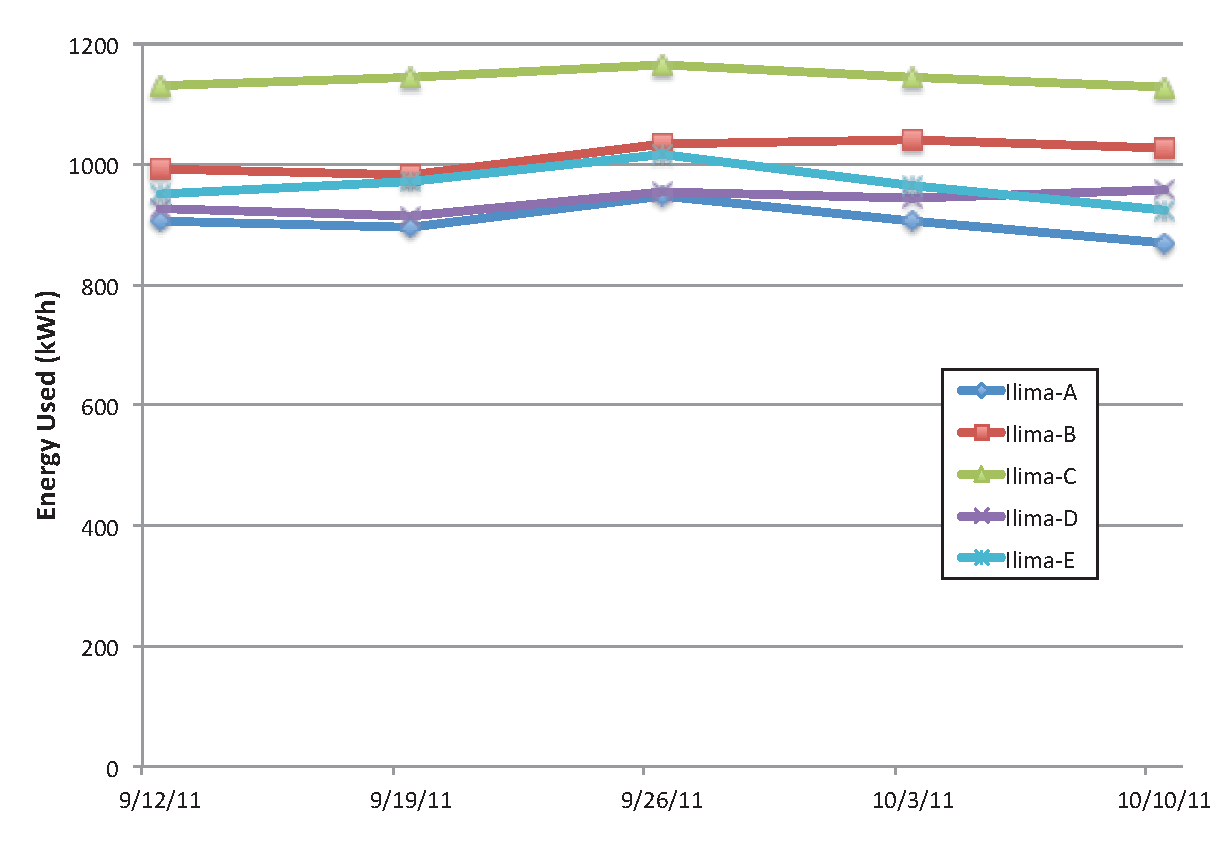
\includegraphics[width=0.8\textwidth]{ilima-before-kwh}
	\caption[Weekly pre-challenge energy use for each lounge in Ilima]{Weekly energy use in kWh for each lounge in Ilima for the pre-challenge period. Dates reflect the start of each week of data.}
	\label{fig:ilima-before-kwh}
\end{figure}

\begin{figure}[htbp]
%% Data from energy-use.xlsx!Baselines
	\centering
	\includegraphics[width=\textwidth]{lehua-before-kwh}
	\caption[Weekly pre-challenge energy use for each lounge in Lehua]{Weekly energy use in kWh for each lounge in Lehua for the pre-challenge period. Dates reflect the start of each week of data.}
	\label{fig:lehua-before-kwh}
\end{figure}

\begin{figure}[htbp]
%% Data from energy-use.xlsx!Baselines
	\centering
	\includegraphics[width=0.8\textwidth]{mokihana-before-kwh}
	\caption[Weekly pre-challenge energy use for each lounge in Mokihana]{Weekly energy use in kWh for each lounge in Mokihana for the pre-challenge period. Dates reflect the start of each week of data.}
	\label{fig:mokihana-before-kwh}
\end{figure}

As the figures show, there can be significant and sustained variation in energy use between lounges, and there can also be significant changes in energy use for a single lounge over time. For example, Ilima C's weekly energy use is consistently over 200\kWh higher than Ilima A or D. Trends over time are sometimes matched between lounges, such as Lehua B and C, but also can be highly divergent such as Mokihana C and E. These differences in energy use over time between lounges show the difficulty in picking a representative baseline from historical data. For example, Mokihana E shows a steep rise in energy use over the two weeks just before the challenge compared to the previous three weeks. The choice of whether to average the three weeks before the challenge or the two weeks before the challenge would have a significant change in Mokihana E's baseline.

For the purposes of evaluation, I used a three-week average of energy use before the challenge for the baselines (see \autoref{sec:baselines-for-analysis}). 

\begin{table}[htbp]
%% Data from "energy-use.xlsx"!"dissertation figures"
	\centering
	\caption{Energy baselines for each lounge used for data analysis.}
	\label{tab:lounge-baselines}
	\vskip 1em
	\begin{tabular}{| l | r |}
		\hline
		Lounge & Baseline (kWh) \\ \hline
		Ilima-A & 908 \\ \hline
		Ilima-B & 1034 \\ \hline
		Ilima-C & 1146 \\ \hline
		Ilima-D & 952 \\ \hline
		Ilima-E & 968 \\ \hline
		Lehua-A & 884 \\ \hline
		Lehua-B & 1063 \\ \hline
		Lehua-C & 913 \\ \hline
		Lehua-D & 872 \\ \hline
		Lehua-E & 861 \\ \hline
		Mokihana-A & 800 \\ \hline
		Mokihana-B & 764 \\ \hline
		Mokihana-C & 933 \\ \hline
		Mokihana-D & 1143 \\ \hline
		Mokihana-E & 1212 \\ \hline
	\end{tabular}
\end{table}


\subsection{During Challenge}

During the challenge, some lounges reduced their energy use, while others increased. \autoref{fig:challenge-kwh} shows the average energy use in kilowatt-hours for each of the 15 lounges during the challenge compared with their baselines.

\begin{figure}[htbp]
%% Data from "energy-use.xlsx"!"dissertation figures"
	\centering
	\includegraphics[width=\textwidth]{challenge-kwh}
	\caption[Baseline energy use compared to challenge energy use for each lounge]{Weekly baseline energy use compared to average weekly energy use during the challenge for each lounge.}
	\label{fig:challenge-kwh}
\end{figure}

Using the baseline, the amount of energy that the 15 lounges would be expected to use is 43,351\kWh for the three week challenge period. The actual energy usage for the 15 lounges during the challenge period was 42,504\kWh, for an overall conservation percentage of 1.95\%.

\autoref{tab:lounge-conservation} shows the percentage of energy conservation on a per-lounge basis. The best lounge (Ilima A) reduced energy use during the challenge by 16.1\% compared to their baseline, but three lounges increased their energy use compared to the baseline during the challenge.

\begin{table}[htbp]
%% Data from "energy-use.xlsx"!"dissertation figures"
	\centering
	\caption[Percentage energy conservation compared to baseline]{Percentage energy conservation compared to baseline for lounges (positive percentages are conservation, negative are increased use).}
	\label{tab:lounge-conservation}
	\vskip 1em
	\begin{tabular}{| l | r |}
		\hline
		Lounge & Conservation \\ \hline
		Ilima-A & 16.1\% \\ \hline
		Ilima-E & 6.4\% \\ \hline
		Lehua-E & 6.1\% \\ \hline
		Lehua-A & 5.5\% \\ \hline
		Ilima-C & 5.3\% \\ \hline
		Mokihana-D & 2.5\% \\ \hline
		Lehua-C & 2.4\% \\ \hline
		Ilima-D & 2.3\% \\ \hline
		Mokihana-E & 2.1\% \\ \hline
		Mokihana-C & 1.5\% \\ \hline
		Ilima-B & 1.3\% \\ \hline
		Lehua-D & 0.5\% \\ \hline
		Mokihana-B & -3.4\% \\ \hline
		Mokihana-A & -8.4\% \\ \hline
		Lehua-B & -11.7\% \\ \hline
	\end{tabular}
\end{table}

Lounges' energy conservation did not seem to be related to the participation rate. \autoref{fig:conservation-vs-participation} shows a chart comparing the percentage energy conservation to the participation rate for each lounge. While the highest conserving lounge (Ilima A, 16.1\%) had the highest participation rate, the second highest participating lounge (Mokihana A) had the second worst energy conservation rate (-8.4\%). The lack of correlation between participation and conservation can be further seen in the scatterplot in \autoref{fig:conservation-vs-participation-scatter}.

\begin{figure}[htbp]
%% Data from "energy-use.xlsx"!"dissertation figures"
	\centering
	\includegraphics[width=\textwidth]{conservation-vs-participation}
	\caption[Percentage energy conservation and participation rate for lounges]{Percentage energy conservation compared to baseline and participation rate for lounges (positive percentages are conservation, negative are increased use). Lounges are sorted from most to least conservation.}
	\label{fig:conservation-vs-participation}
\end{figure}

\begin{figure}[htbp]
%% Data from "Energy-scatterplots.xlsx"!"dissertation charts"
	\centering
	\includegraphics[width=0.8\textwidth]{conservation-vs-participation-scatter}
	\caption[Scatterplot of percentage energy conservation and participation rate for lounges]{Scatterplot of percentage energy conservation compared to baseline and participation rate for lounges (positive percentages are conservation, negative are increased use).}
	\label{fig:conservation-vs-participation-scatter}
\end{figure}

Total lounge score also does not appear to be correlated with conservation. \autoref{fig:conservation-vs-score-scatter} shows a scatterplot of lounge conservation and score.

\begin{figure}[htbp]
%% Data from "Energy-scatterplots.xlsx"!"dissertation charts"
	\centering
	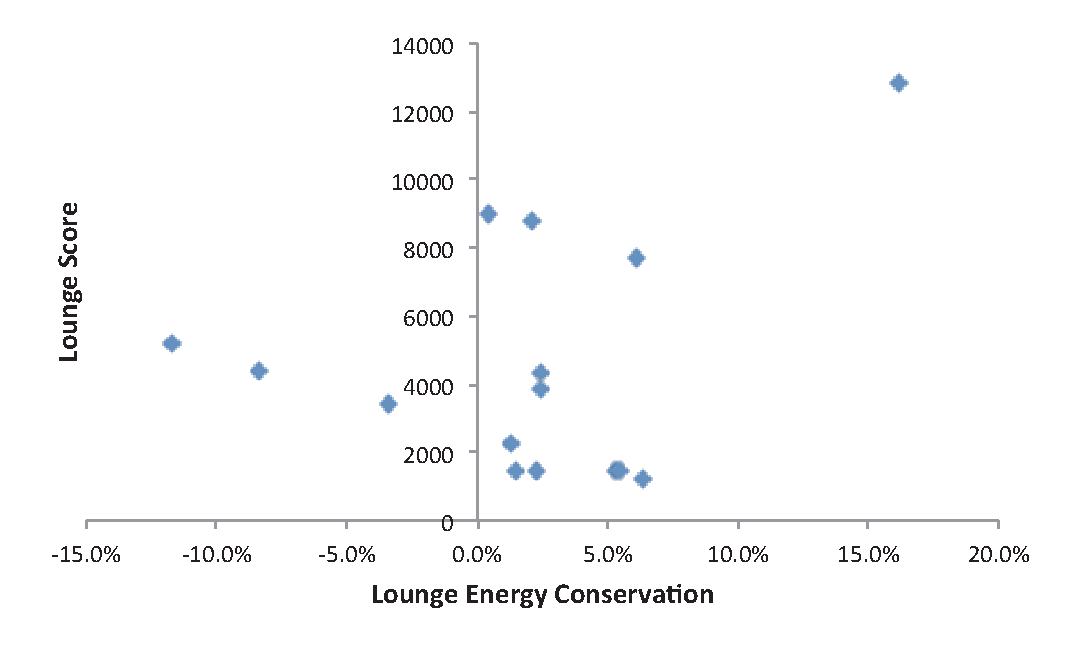
\includegraphics[width=0.8\textwidth]{conservation-vs-score-scatter}
	\caption[Scatterplot of percentage energy conservation and score for lounges]{Scatterplot of percentage energy conservation compared to baseline and total score for lounges (positive percentages are conservation, negative are increased use).}
	\label{fig:conservation-vs-score-scatter}
\end{figure}

While there is no obvious trend between lounge score or participation and conservation, it is worth noting that the lounge with the highest score had the highest participation, and the highest conservation. Based on informal discussions with members of this team at events and award parties, it was clear that this winning lounge was highly motivated to win and was taking active measures to reduce energy use.


\subsection{After Challenge}

Energy monitoring continued throughout the post-challenge period until the end of the spring 2012 semester. \autoref{fig:after-average-energy} shows the weekly energy use averaged across all lounges during the post-challenge period. As can clearly be seen, there are large drops in energy use during five periods: Thanksgiving week, fall finals, winter break, spring break, and spring finals. These drops are expected, as many students use these periods as opportunities to travel or return to their homes. \autoref{fig:after-average-energy} clearly shows the impact that changes in occupancy have on energy use in Hale Aloha. While these five periods are predictable because they are scheduled on the university calendar, in general, changes to occupancy are difficult to measure directly. Official rosters from Student Housing only reflect an approximation of occupancy, because residents can move unofficially between rooms without approval or notification to Housing. For example, during the post-challenge energy audit (described in \autoref{sec:post-energy-audit}), four beds were found in one room that was intended for two residents. Occupancy changes are difficult to track, yet can have a major impact on energy use.

\begin{figure}[htbp]
%% Data from "energy-use.xlsx"!"dissertation figures"
	\centering
	\includegraphics[width=\textwidth]{after-average-energy}
	\caption{Energy use averaged across all lounges during post-challenge period.}
	\label{fig:after-average-energy}
\end{figure}

Because these five periods of known lower occupancy reduce energy use, I have removed them from the analyses of energy use in the rest of this section. \autoref{fig:ilima-after-kwh}, \autoref{fig:lehua-after-kwh}, and \autoref{fig:mokihana-after-kwh} show the energy use in kilowatt-hours for Ilima, Lehua, and Mokihana respectively for the post-challenge period, with the low-occupancy periods removed. As was seen in the pre-challenge period, there is considerable variation in energy use between lounges, but there are no clear patterns of post-challenge energy use.

\begin{figure}[htbp]
%% Data from "energy-use.xlsx"!"dissertation after"
	\centering
	\includegraphics[width=\textwidth]{ilima-after-kwh}
	\caption[Weekly post-challenge energy use for each lounge in Ilima]{Weekly energy use in kWh for each lounge in Ilima for the post-challenge period, with weeks of low occupancy removed. Dates reflect the start of each week of data.}
	\label{fig:ilima-after-kwh}
\end{figure}

\begin{figure}[htbp]
%% Data from "energy-use.xlsx"!"dissertation after"
	\centering
	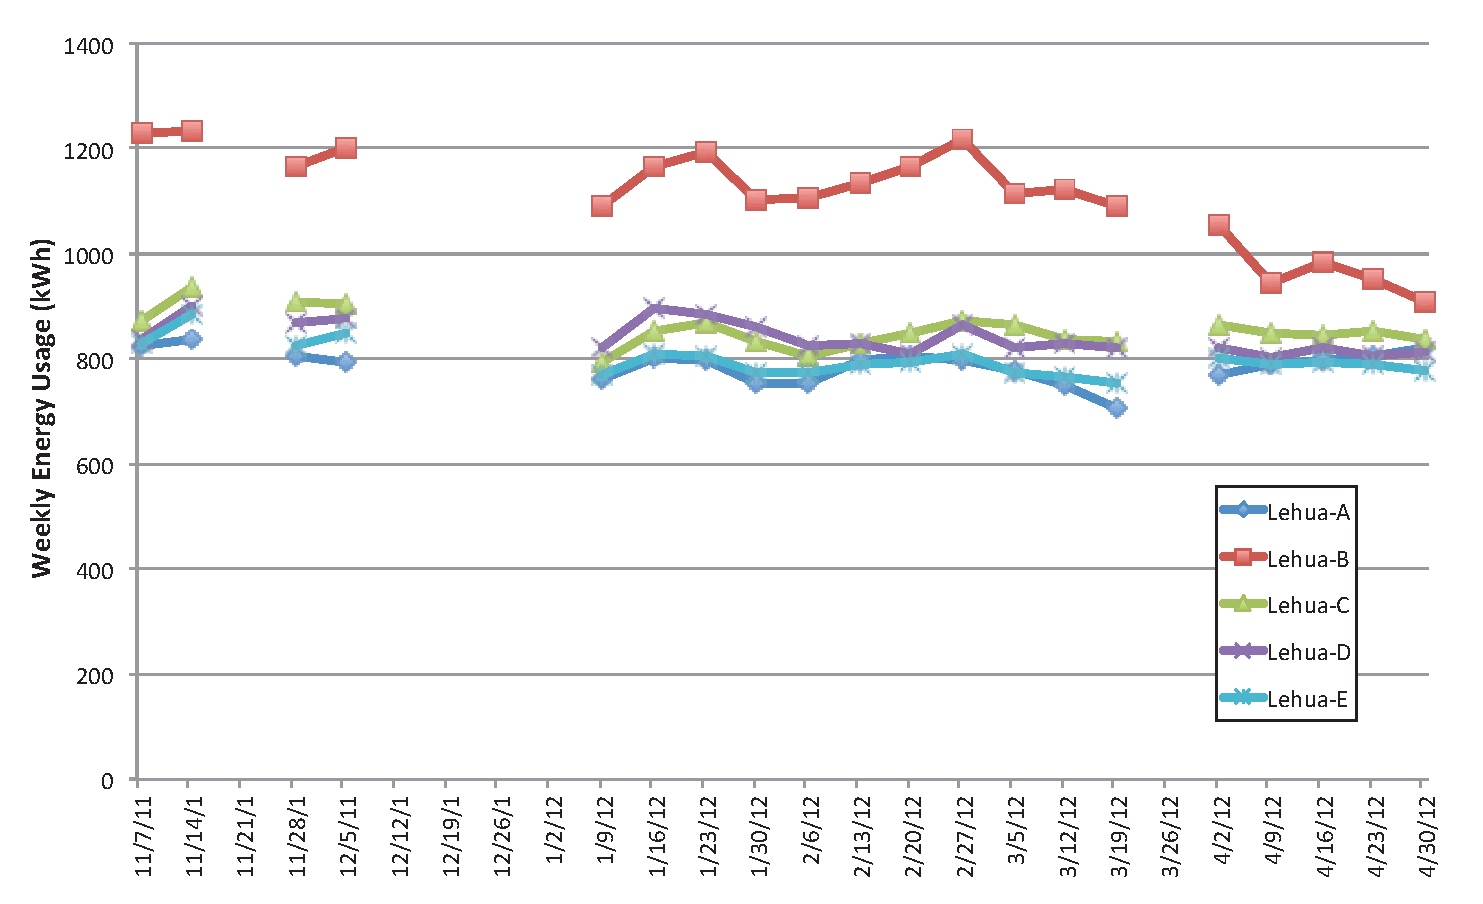
\includegraphics[width=\textwidth]{lehua-after-kwh}
	\caption[Weekly post-challenge energy use for each lounge in Lehua]{Weekly energy use in kWh for each lounge in Lehua for the post-challenge period, with weeks of low occupancy removed. Dates reflect the start of each week of data.}
	\label{fig:lehua-after-kwh}
\end{figure}

\begin{figure}[htbp]
%% Data from "energy-use.xlsx"!"dissertation after"
	\centering
	\includegraphics[width=\textwidth]{mokihana-after-kwh}
	\caption[Weekly post-challenge energy use for each lounge in Mokihana]{Weekly energy use in kWh for each lounge in Mokihana for the post-challenge period, with weeks of low occupancy removed. Dates reflect the start of each week of data.}
	\label{fig:mokihana-after-kwh}
\end{figure}

\autoref{fig:ilima-after-percent}, \autoref{fig:lehua-after-percent}, and \autoref{fig:mokihana-after-percent} show the energy use for Ilima, Lehua, and Mokihana in the post-challenge period as a percentage change from the baseline. As mentioned earlier, energy use in the post-challenge period was wildly variable, but there are several notable points. Ilima A, the lounge that reduced their energy use the most during the challenge, did not maintain that reduction throughout the post-challenge period (see \autoref{fig:ilima-after-percent}). During the remainder of the fall 2011 semester, Ilima A's energy use was below its baseline, but it was higher than during the challenge itself. However, in the spring 2012 semester, Ilima A's energy use increases above the baseline value for most of the semester.

\begin{figure}[htbp]
%% Data from "energy-use.xlsx"!"dissertation after"
	\centering
	\includegraphics[width=0.9\textwidth]{ilima-after-percent}
	\caption[Percentage post-challenge energy use difference from baseline for Ilima]{Percentage difference for weekly post-challenge energy use compared to baseline for each lounge in Ilima, with weeks of low occupancy removed (positive percentages are increased use, negative are reduced use). Dates reflect the start of each week of data.}
	\label{fig:ilima-after-percent}
\end{figure}

The five lounges of Lehua show an interesting pattern of parallel changes in energy use compared to their baseline during the spring 2012 semester until spring break (\autoref{fig:lehua-after-percent}). Neither of the other two towers show this same pattern across all lounges.

\begin{figure}[htbp]
%% Data from "energy-use.xlsx"!"dissertation after"
	\centering
	\includegraphics[width=0.9\textwidth]{lehua-after-percent}
	\caption[Percentage post-challenge energy use difference from baseline for Lehua]{Percentage difference for weekly post-challenge energy use compared to baseline for each lounge in Lehua, with weeks of low occupancy removed (positive percentages are increased use, negative are reduced use). Dates reflect the start of each week of data.}
	\label{fig:lehua-after-percent}
\end{figure}

One dramatic change is the reduction in energy use by Mokihana C during the spring 2012 semester (\autoref{fig:mokihana-after-percent}). Mokihana C's energy use quickly dropped by 40\% compared to its baseline in the week of 1/23/12, and stays around this level for the remainder of the semester. I noticed this change in February 2012, and asked the RD for Mokihana whether there had been any changes in occupancy or appliances (such as the removal of in-room air conditioners) that could account for the change. The RD and RAs indicated that there were no such changes that they were aware of, so it is unclear what caused this change in energy use.

\begin{figure}[htbp]
%% Data from "energy-use.xlsx"!"dissertation after"
	\centering
	\includegraphics[width=0.9\textwidth]{mokihana-after-percent}
	\caption[Percentage post-challenge energy use difference from baseline for Mokihana]{Percentage difference for weekly post-challenge energy use compared to baseline for each lounge in Ilima, with weeks of low occupancy removed (positive percentages are increased use, negative are reduced use). Dates reflect the start of each week of data.}
	\label{fig:mokihana-after-percent}
\end{figure}


\subsection{Discussion}
\label{sec:energy-result-discussion}

Research question \#3 is ``how did energy use change during the challenge?'' Based on the data presented in this section, some lounges reduced their energy use during the challenge, while others increased their usage. For a lounge to reduce its energy usage, its residents need to make concerted changes to their behavior. If the Kukui Cup is the facilitator of the behavior changes, then residents will participate in the Kukui Cup game experience by earning points. However, \autoref{fig:conservation-vs-participation} and \autoref{fig:conservation-vs-participation-scatter} show that participation alone is not sufficient to ensure energy conservation. While the lounge that conserved the most during the challenge also had the highest participation, participation did not lead to conservation in other cases.

One possible reason for the lack of greater energy conservation relates to our use of lounges as the team unit for the 2011 UH Kukui Cup. Lounges consist of a fairly large group of 54 residents, and since they are split across two floors, some lounge members may only rarely see residents that live on the other floor of the lounge. While the shared lounge space and lounge-level elevator create some potential for interaction between the two floors, the choice of the lounge as team was forced by electrical infrastructure in Hale Aloha. The results of the group identification scale further show that residents do not strongly identify with their lounge, and in some cases may not even be aware of the lounge concept. These factors work against the type of esprit de corps needed for a team to pull together and make changes in behavior as a group.

Research question \#4 is ``how did energy use change after the challenge?''. Post-challenge energy use varied substantially over time and across lounges, even after accounting for predictable occupancy changes. There is no evidence of any sustained change in behavior, as reflected in energy use. The lounge that conserved the most energy during the challenge failed to maintain that conservation through the rest of the academic year. Further, given the variation in energy use over time, it seems unlikely that one could tease out the impact of the Kukui Cup from all the other factors that could influence energy use such as temporary changes in occupancy, weather patterns, and semester schedules.

Finally, these results bring to light the multifaceted problems with using energy baselines as a means of evaluating the effect of energy competitions or other energy interventions. The two primary ways of computing baselines are: averaging energy data for the challenge period from previous years, and averaging data from weeks before the start of the challenge.

Averaging data from previous years exposes the baseline to any changes in building infrastructure that may have taken place. As energy prices rise and building operation budgets tighten, building managers are increasingly investing in infrastructure improvements that reduce energy use such as more efficient lighting, heating and cooling, or increased insulation. Weather changes between years could also dramatically affect baseline calculations, making them poor predictors of energy use.

Using energy data collected shortly before the challenge sidesteps some of the problems from previous year data, such as changes in weather and building infrastructure, but creates new problems. Creating a baseline using only two or three weeks of data magnifies the impact of any anomalous activity that changes energy use. When energy use has a clear trend upward or downward during the period being averaged, the baseline will smooth out that trend. For example, in \autoref{fig:mokihana-before-kwh}, Mokihana E's energy increases substantially during the two weeks before the challenge. If this increase reflects a permanent change to the lounge's energy use (such new residents moving in), then a baseline computed from three weeks of data will lower the baseline, making it an inaccurate predictor of future use and making it harder for Mokihana C to win any competition using that baseline. If the increase is a temporary change (abnormally warm weather or out-of-town guests visiting), then a three-week baseline will be higher than it should be to predict future use and make it easier for Mokihana C to perform well in a competition. In short, there are many possible causes of changes in energy use during the baseline period, and without deep insight into those changes, the choice of a particular baseline computation method will be arbitrary and likely inaccurate. Using baselines to assess long-term changes in behavior are even more problematic, as the further away in time from the baseline period one gets, the less likely the baseline is to be an accurate predictor of energy use.

The arbitrariness of baselines can be further demonstrated through problems Oberlin College encountered during the 2010 Campus Conservation Nationals~\cite{Willens2010}. During the first two weeks of the competition, Oberlin had a 5\% increase in electricity use, which led to a ranking of 32nd place, which is surprising since Oberlin was a leader in campus energy competitions~\cite{petersen-dorm-energy-reduction}. The poor ranking led to frustration among some student participants, one of whom is quoted as saying ``We've turned off every fucking light in this building, dude, and it's not making a goddamn difference.'' Oberlin challenge organizers felt that the baseline was not accurate: ``During the competition, it became clear that this common baseline period \ldots was, in some cases, resulting in percentage changes for individual buildings and sometimes for whole campuses that were more attributable to changes in weather and other factors than to the choices that students were making in their dorms''. After discussing with the national competition organizers, the baseline was changed (presumably increased) ``for schools with resource increases greater than 15 percent''. While there is little doubt that the Oberlin challenge organizers felt there were good reasons for changing the baseline, these reasons only came to light because Oberlin was faring poorly in the competition. Since there is little justification for picking a particular baseline, it is easy for competition organizers to pick them in such a way that competitions are found to be successful in spurring energy conservation through behavior change.

Since baselines form the basis for evaluating energy competitions, these fundamental problems with computing baselines call into question the published results from all competitions. Further, the problems with baselines are not discussed in the literature. The articulation of these issues with baselines is one of the major contributions of this research.


\section{Action Effectiveness}

Research question \#6 is ``how effective were the actions available via the website?'' One measure of the effectiveness of the actions is to examine their relationship with energy literacy. Since only 24 subjects completed both pre- and post-challenge energy literacy questionnaires, the effectiveness of the actions on energy literacy levels will be limited to that data. My hypothesis is that participation in the challenge (as evidenced by score and actions completed) would correlate with improvement in energy knowledge.

\autoref{tab:knowledge-delta-participant} shows the change in the number of energy knowledge questions answered correctly from the pre-challenge questionnaire to the post-challenge questionnaire, along side the participants' scores and the number of actions they completed. For comparison, \autoref{tab:knowledge-delta-nonparticipant} shows the changes for non-participants.

\begin{table}[htbp]
%% Data from "SurveyExport.xlsx"!"RQ6 data"
	\centering
	\caption[Changes in energy knowledge for challenge participants]{Change in number of energy knowledge questions answered correctly between pre- and post-challenge questionnaires for challenge participants, compared to score and number of actions completed.}
	\label{tab:knowledge-delta-participant}
	\vskip 1em
	\begin{tabular}{| c | r | r | r | r | r |}
		\hline
		Participant \# & Knowledge $\Delta$ & Pre & Post & Points & Actions completed \\ \hline
		1 & 7 & 8 & 15 & 1154 & 61\\ \hline
		2 & 7 & 6 & 13 & 405 & 28\\ \hline
		3 & 5 & 6 & 11 & 260 & 27\\ \hline
		4 & 5 & 6 & 11 & 45 & 1\\ \hline
		5 & 5 & 9 & 14 & 1279 & 69\\ \hline
		6 & 3 & 5 & 8 & 248 & 23\\ \hline
		7 & 3 & 8 & 11 & 357 & 22\\ \hline
		8 & 3 & 2 & 5 & 45 & 2\\ \hline
		9 & 3 & 5 & 8 & 297 & 17\\ \hline
		10 & 2 & 6 & 8 & 25 & 1\\ \hline
		11 & 2 & 10 & 12 & 105 & 9\\ \hline
		12 & 2 & 7 & 9 & 45 & 2\\ \hline
		13 & 2 & 6 & 8 & 65 & 2\\ \hline
		14 & 1 & 12 & 13 & 385 & 28\\ \hline
		15 & 0 & 6 & 6 & 355 & 28\\ \hline
		16 & 0 & 7 & 7 & 110 & 5\\ \hline
		17 & -1 & 13 & 12 & 295 & 28\\ \hline
		18 & -1 & 10 & 9 & 642 & 43\\ \hline
		19 & -1 & 9 & 8 & 512 & 38\\ \hline
		20 & -2 & 11 & 9 & 85 & 2\\ \hline
		21 & -2 & 5 & 3 & 45 & 3\\ \hline
		22 & -3 & 6 & 3 & 25 & 1\\ \hline
		23 & -3 & 8 & 5 & 35 & 2\\ \hline
		24 & -3 & 10 & 7 & 105 & 1\\ \hline	\end{tabular}
\end{table}

\begin{table}[htbp]
%% Data from "SurveyExport.xlsx"!"RQ6 data"
	\centering
	\caption[Changes in energy knowledge for non-challenge participants]{Change in number of energy knowledge questions answered correctly between pre- and post-challenge questionnaires for non-challenge participants.}
	\label{tab:knowledge-delta-nonparticipant}
	\vskip 1em
	\begin{tabular}{| c | r | r | r |}
		\hline
		Participant \# & Knowledge $\Delta$  & Pre & Post\\ \hline
		25 & 3 & 5 & 8\\ \hline
		26 & 2 & 7 & 9\\ \hline
		27 & 2 & 6 & 8\\ \hline
		28 & 2 & 9 & 11\\ \hline
		29 & 2 & 9 & 11\\ \hline
		30 & 2 & 7 & 9\\ \hline
		31 & 1 & 3 & 4\\ \hline
		32 & 1 & 6 & 7\\ \hline
		33 & 1 & 7 & 8\\ \hline
		34 & 1 & 8 & 9\\ \hline
		35 & 1 & 8 & 9\\ \hline
		36 & 1 & 4 & 5\\ \hline
		37 & 0 & 6 & 6\\ \hline
		38 & 0 & 6 & 6\\ \hline
		39 & 0 & 5 & 5\\ \hline
		40 & -1 & 9 & 8\\ \hline
		41 & -1 & 5 & 4\\ \hline
		42 & -1 & 8 & 7\\ \hline
		43 & -1 & 8 & 7\\ \hline
		44 & -2 & 9 & 7\\ \hline
		45 & -2 & 9 & 7\\ \hline
		46 & -3 & 10 & 7\\ \hline
		47 & -4 & 12 & 8\\ \hline
		48 & -6 & 13 & 7\\ \hline
	\end{tabular}
\end{table}

\autoref{fig:knowledge-vs-score} is a scatterplot of the change in energy knowledge questions answered correctly against the participant's score. While the plot shows two data points in the upper right hand quadrant representing high scores and large improvements, the overall trend is unclear. There is substantial variation in the knowledge change among low-scoring participants, perhaps indicating that light participation in the Kukui Cup does not have much impact on energy knowledge.

\begin{figure}[htbp]
%% Data from "SurveyExport.xlsx"!"RQ6 data"
	\centering
	\includegraphics[width=0.95\textwidth]{knowledge-vs-score}
	\caption[Scatterplot of change in energy knowledge and participant score]{Scatterplot of change in number of energy knowledge questions answered correctly between pre and post-challenge questionnaires for challenge participants, compared to score.}
	\label{fig:knowledge-vs-score}
\end{figure}

Since we assigned scores to actions based on guesses of how effective they might be (see \autoref{sec:point-appropriateness} for more discussion), using total score as the indicator of participation might not fully reflect participation. \autoref{fig:knowledge-vs-actions} is a similar scatterplot, showing change in energy knowledge questions answered correctly, but plotted against the number of actions a participant completed. The results are quite similar to the score scatterplot; therefore, score seems to be a reasonable assessment of a participant's degree of participation.

\begin{figure}[htbp]
%% Data from "SurveyExport.xlsx"!"RQ6 data"
	\centering
	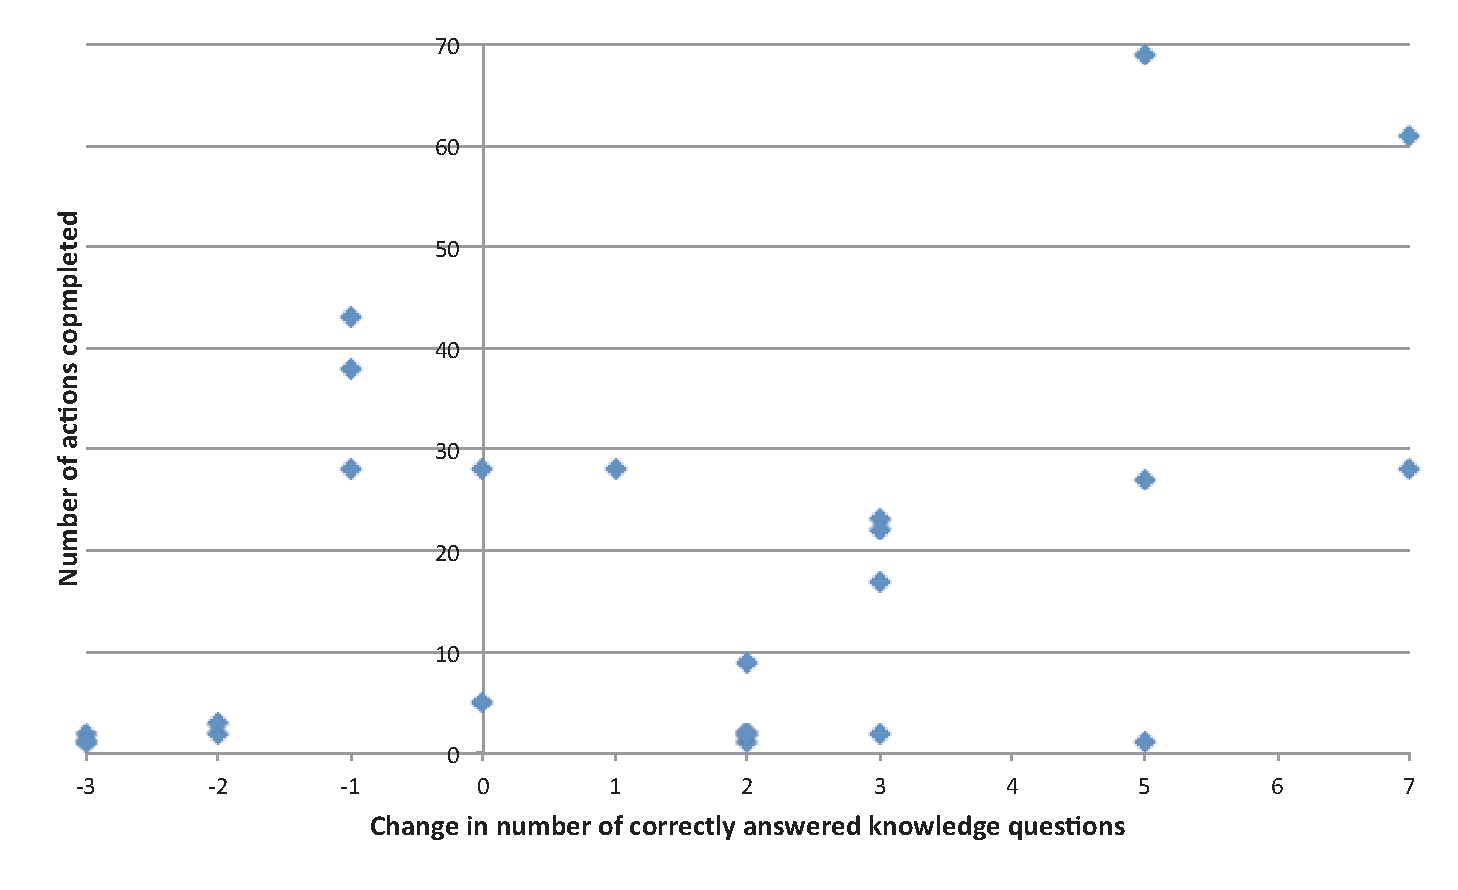
\includegraphics[width=0.95\textwidth]{knowledge-vs-actions}
	\caption[Scatterplot of change in energy knowledge and actions completed]{Scatterplot of change in number of energy knowledge questions answered correctly between pre and post-challenge questionnaires for challenge participants, compared to number of actions completed by participant.}
	\label{fig:knowledge-vs-actions}
\end{figure}

Plots based on \emph{change} in energy knowledge do not account for players that might already know about energy, since they might see little or no change in their energy literacy despite playing the game. \autoref{fig:post-challenge-vs-score} is a scatterplot showing participants post-challenge energy knowledge score plotted against their score. While constrained by the sample size, there are no data points that contradict the hypothesis that participating in the challenge increases energy literacy. All the data points lie to the right of a diagonal line drawn from lower left to upper right, showing that as players earned more points, they were more likely to score better on the energy knowledge questions.

\begin{figure}[htbp]
%% Data from "SurveyExport.xlsx"!"RQ6 data"
	\centering
	\includegraphics[width=0.95\textwidth]{post-challenge-vs-score}
	\caption[Scatterplot of post-challenge energy knowledge and participant score]{Scatterplot of post-challenge energy knowledge questions answered correctly for challenge participants, compared to score.}
	\label{fig:post-challenge-vs-score}
\end{figure}

Based on the limited data available, it is unclear how effective the individual actions available in the challenge were to increasing energy knowledge. However, I did not find any evidence that contradicts the conclusion that the more points earned and actions completed, the higher the participant's post challenge energy literacy score.


\section{Action Point Value Appropriateness}
\label{sec:point-appropriateness}

Research question \#7 is ``how appropriate were the point values assigned to actions?'' As described in \autoref{sec:exp-point-values}, we assigned points to actions primarily based on the expected difficulty of the action, and a guess as to how effective they might be at increasing energy literacy. \autoref{tab:point-rubric2} shows the general rubric we used for assigning point values to actions.

\begin{table}[htbp]
	\centering
	\caption{List of point categories for actions (repeated from \autoref{tab:point-rubric})}
	\label{tab:point-rubric2}
	\vskip 1em
	\begin{tabular}{| c | l | c |}
		\hline
		Point value & Type of action & Time commitment \tabularnewline \hline \hline
		5 & Tweet something or complete a commitment & 1--2 min \\ \hline
		10 & Watch tutorial video, slightly more involved activities & 5 min \\ \hline
		20 & Attend an event & 1--2 hours \\ \hline
		30 & Priority events or activities & 10--60 min \\ \hline
		5--50 & Creative activities (e.g.\ writing a letter to editor) & multiple hours \\ \hline
	\end{tabular}
\end{table}

One issue with this point rubric is that the range is quite narrow, and point values do not scale with the expected amount of time required to complete the action. For example, sending a tweet with Twitter might take one minute for 5 points, but creating a video about the Kukui Cup could take hours and has a maximum potential of 50 points (for an excellent video). This disparity was also a concern for events, which required attendance at a particular time and place, often for an hour or more, but were often worth only 20 points. Making points scale more linearly with the expected time commitment would better balance the rubric. Off-campus excursions were poorly attended during the challenge. The attendance level could have partly been due to their low point values compared to player's investment in time to attend them.

One measure of the appropriateness of questions is the number of rejected submissions from players compared to the number of completions. \autoref{tab:action-rejection} shows the activities that had a rejection rate above 20\% based on the total number of activity submissions that were accepted compared to those that were rejected.

\begin{table}[htbp]
%% Data from "activities-rejections.xlsx"!"rejections"
	\centering
	\small
	\caption{A list of activities with rejection rate above 20\%}
	\label{tab:action-rejection}
	\vskip 1em
	\begin{tabular}{| l | r | r | r | r |}
		\hline
		Activity & Points & Completions & Rejections & Reject rate \\ \hline
		Make a video on a Kukui Cup topic & 5--50 & 4 & 3 & 75\% \\ \hline
		Refer a friend to the Kukui Cup & 5 & 12 & 6 & 50\% \\ \hline
		Write a song about a Kukui Cup topic & 5--50 & 2 & 1 & 50\% \\ \hline
		Learn more about opala & 15 & 31 & 14 & 45\% \\ \hline
		Watch video about Power \& Energy & 10 & 198 & 80 & 40\% \\ \hline
		Share Kukui Cup link on Google+ & 5 & 45 & 15 & 33\% \\ \hline
		Label power hogs in your room & 15 & 22 & 7 & 32\% \\ \hline
		Learn more about transportation & 15 & 69 & 19 & 28\% \\ \hline
		Learn more about the Hawaii Clean Energy Init. & 15 & 33 & 8 & 24\% \\ \hline
		Play the photo chain game & 10 & 22 & 5 & 23\% \\ \hline
		Watch video on Energy Intuition & 10 & 147 & 29 & 20\% \\ \hline
%		Watch video about solar energy & 10 & 51 & 9 & 18\% \\ \hline
%		Watch video about Lighting & 10 & 138 & 24 & 17\% \\ \hline
%		Learn more about Energy Intuition & 15 & 70 & 11 & 16\% \\ \hline
%		Learn more about climate change & 15 & 51 & 8 & 16\% \\ \hline
%		Measure sink water flow & 15 & 15 & 2 & 13\% \\ \hline
%		Estimate your room's total daily energy use & 35 & 16 & 2 & 13\% \\ \hline
%		Write a letter to the editor on a Kukui Cup topic & 5--50 & 8 & 1 & 12\% \\ \hline
%		Learn more about solar energy & 15 & 25 & 3 & 12\% \\ \hline
	\end{tabular}
\end{table}

The first and third activities in the table are from the creative category, and already have the a high point value as the top end of the variable range. As discussed earlier in this section, higher point values for activities that require a greater time investment would be worthwhile. The second activity was intended to encourage players to refer new players to the game using the referral bonus. The referral bonus was confusing to some players who sometimes thought they had referred new players when they had not done so. However, confusion with the referral bonus is best handled by through the referral bonus mechanism directly and not by increasing the value of this ancillary activity.

Some of the activities in the in table refer to watching a video, and we created most of these videos. Those videos that had high rejection rates probably reflect confusing videos that could be improved by creating better videos, or switching to another means of communicating the information. For example, many players had problems understanding the difference between power and energy. While this can be a tricky concept, it also might be better understood through an interactive game or display where players can explore the two concepts by turning on and off electricity to different virtual appliances.

The Google+ link sharing activity was intended only as a way to increase awareness of the Kukui Cup, but at the time of the challenge, Google+ was a new service and not as easy to share content compared to Facebook and Twitter. This activity could easily be removed with no negative impact on the challenge. Labelling appliances with their energy use (``Label power hogs in your room'') required more effort than comparable 15 point activities, so its point value should be increased.

Overall, it appears that the point rubric we used was appropriate, with the exception of not providing enough points for events, which had a higher time investment than most other actions.


\section{Importance of Lounge-Level Feedback}

Research question \#8 is ``how important was lounge-level near-realtime feedback?'' Lounge-level feedback was integrated into the challenge in several ways including: the energy competition, the Daily Energy Goal Game, and two different types of lounge-level energy prizes per round.

There was only one activity (excluding Canopy activities) that required players to use the lounge-level energy data: ``Examine your lounge's energy use''. To complete this activity, players had to view the Go Low page that contained the energy data and report back on ``is your lounge above or below the energy goal, by how much, and name one activity that might help your lounge conserve energy.'' 95 players completed this activity, which is 23.6\% of the participants in the challenge. This percentage is quite close to the 25\% threshold I established in \autoref{sec:exp-lounge-level}.

In the final round of the challenge, we provided players with an online survey that they could complete for 40 points. \autoref{app:in-game-questionnaire} provides a list of the questions in the survey. 43 players completed the survey. One of the questions in the survey was ``The Kukui Cup website shows energy data updated every 15 seconds. Did you find this helpful in conserving energy?''. \autoref{tab:survey-real-time-energy} shows the results.

\begin{table}[htbp]
	\centering
	\caption[Survey response on helpfulness of real-time energy data]{Survey answers to the question ``The Kukui Cup website shows energy data updated every 15 seconds. Did you find this helpful in conserving energy?''}
	\label{tab:survey-real-time-energy}
	\vskip 1em
	\begin{tabular}{| l | r | r |}
		\hline
		Answer & Count & Percentage \tabularnewline \hline \hline
		not really, updating the data daily would be enough & 2 & 4.7\% \\ \hline
		not really, updating the data hourly would be enough & 7 & 16.3\% \\ \hline
		not really, I only care about the final result of the competition & 2 & 4.7\% \\ \hline
		yes, it is helpful to see the energy usage changing in real time & 32 & 74.4\% \\ \hline
	\end{tabular}
\end{table}

The in-game survey suffers from some limitations: it did not come from a random sample of players, players were incentivized to participate using points, and players may have felt that giving positive responses would curry favor with the administrators and thereby help them in the challenge. Given these limitations, survey respondents did report that the real-time lounge-level energy feedback was helpful by a wide margin.

Based on the results presented here, the case for lounge-level feedback is not clear cut. Providing feedback at a finer grain than an entire building enables a variety of possibilities in a challenge such as floor versus floor competitions and energy goals. However, it at least in the case of Hale Aloha, players do not strongly identify with their floor (as discussed in \autoref{sec:group-id}), making the utility of floor competitions unclear. It is possible that with smaller team units, or teams built around groups that players identify more strongly, the problems we experienced in Hale Aloha might not occur.

The case for providing real-time data, which requires effort and expense beyond the lounge-level metering, is less clear. The only game component in the challenge that required real-time feedback was the Current Power widget (see \autoref{sec:go-low-page}). The inclusion of this widget on the Go Low webpage provides an element that updates every 15 seconds, which adds to the visual interest of the page. While the Current Power widget was originally conceived as a way for players to experiment with how much energy their devices use, we have no evidence that players actually did experiment in this way. Since the energy data is aggregated across 54 residents, only fairly large loads (such as microwaves) are likely to be visible amongst the noise of other loads being turned on and off. However, 74\% of the players responding to the in-game survey indicated that they found the rapidly-updated energy data helpful, which is a positive factor in considering whether to provide real-time data in energy competitions.


\section{Post-Challenge Energy Audit}
\label{sec:post-energy-audit}

As described in \autoref{sec:meter-installation}, installation of the electricity meters for the challenge was completed during the Fall 2011 semester. A joint team from UH \Manoa Student Housing and the Kukui Cup project conducted an energy audit of the four Hale Aloha towers during the winter break after the Fall 2011 semester~\cite{csdl2-11-12}\fxnote{Maybe should put this report into an appendix to be self-contained?}. Residents are not required to leave during the winter break, but many residents do leave, providing an opportunity to unplug all devices in resident rooms and examine the power usage recorded by the lounge meters. The power usage results are discussed in \autoref{sec:panel-audits}. However, Housing had these additional goals for the audit:

\begin{enumerate}
\item Making a count of the types of appliances residents have in their rooms.
\item Unplugging unused \& unneeded appliances for residents who were away for winter break to conserve energy.
\item Noting any violations of rules, such as attaching things to fire sprinkler heads, or having an unapproved air conditioner.
\end{enumerate}

It is likely that some residents that left during the winter break took some portable appliances with them, such as laptops, and might have moved out ``contraband'' appliances. Therefore, the appliance count will probably be an underestimate of what was actually present during the Fall 2011 semester.


\subsection{Auditing Procedure}

The four Hale Aloha towers were audited between December 19 to December 22, auditing lounge by lounge using the following procedure:

\begin{itemize}
	\item One team examined each room on the first floor of the lounge. They recorded the appliances present in the room on a worksheet.
	\item For unoccupied rooms, all appliances were unplugged.
	\item For occupied rooms, the resident was asked to unplug all devices until the audit is complete.
	\item Once everything has been unplugged, we examined the power readings on the two meters that monitor each lounge. Using the electrical panel that each meter is attached to, we turned off each circuit breaker and recorded any change in power use from the meter display.
\end{itemize}


\subsection{Appliance Count}
\label{sec:appliance-count}

The energy audit also produced a list of the number of appliances in each room. \autoref{tab:appliance-count} shows the total number of appliances per tower, while \autoref{tab:appliance-average} shows the average number of appliances per room for each tower.

\begin{table}[htbp]
	\centering
	\caption{Total appliance count per tower}
	\label{tab:appliance-count}
	\vskip 1em
		\begin{tabular}{| c || c | c | c | c | c | c | c |}
			\hline
			Tower & Microwaves & Desktop Computers & Laptops & Fans & Lamps & TVs & Printers \tabularnewline \hline \hline
			
			Lehua & 120 & 5 & 25 & 224 & 96 & 69 & 150 \tabularnewline \hline

			Ilima & 103 & 2 & 44 & 273 & 93 & 79 & 131 \tabularnewline \hline

			Lokelani & 86 & 2 & 48 & 273 & 121 & 67 & 139 \tabularnewline \hline

			Mokihana & 89 & 18 & 43 & 252 & 88 & 68 & 129  \tabularnewline \hline

		\end{tabular}
\end{table}

\begin{table}[htbp]
	\centering
	\caption{Average number of appliances per room for each tower}
	\label{tab:appliance-average}
	\vskip 1em
		\begin{tabular}{| c || c | c | c | c | c | c | c |}
			\hline
			Tower & Microwaves & Desktop Computers & Laptops & Fans & Lamps & TVs & Printers \tabularnewline \hline \hline
			
			Lehua & 0.86 & 0.04 & 0.18 & 1.60 & 0.69 & 0.49 & 1.07 \tabularnewline \hline

			Ilima & 0.74 & 0.01 & 0.31 & 1.95 & 0.66 & 0.56 & 0.94 \tabularnewline \hline

			Lokelani & 0.61 & 0.01 & 0.34 & 1.95 & 0.86 & 0.48 & 0.99 \tabularnewline \hline

			Mokihana & 0.64 & 0.13 & 0.31 & 1.80 & 0.63 & 0.49 & 0.92 \tabularnewline \hline

		\end{tabular}
\end{table}

From these counts, we see that most rooms have a printer, and that microwaves and TVs are quite popular. The count of laptops is likely a major underestimate since many residents were away for the break, and likely took their laptop with them. We did record a laptop when there was some evidence that a laptop was usually present (such as a laptop stand, mouse pad, or power adapter). Desktop computers seem to be quite rare, presumably displaced by laptop usage.

A surprising finding was the prevalence of mini refrigerators. \autoref{tab:fridge-distribution} shows the distribution of refrigerators across the four towers.

\begin{table}[htbp]
	\centering
	\caption{Refrigerator distribution by tower}
	\label{tab:fridge-distribution}
	\vskip 1em
		\begin{tabular}{| c || c | c | c | c | c | c |}
			\hline
			Tower & \# fridges & avg.\ fridges/room & 0 fridges & 1 fridge & 2 fridges & 3 fridges \tabularnewline \hline \hline
			
			Mokihana & 149 & 1.06 & 19 & 93 & 28 & 0  \tabularnewline \hline
			
			Lehua & 176 & 1.26 & 7 & 90 & 43 & 0 \tabularnewline \hline
			
			Ilima & 176 & 1.26 & 7 & 91 & 41 & 1 \tabularnewline \hline

			Lokelani & 177 & 1.26 & 12 & 79 & 49 & 0 \tabularnewline \hline

		\end{tabular}
\end{table}

We see that most rooms have a refrigerator, and many have two. Based on this, it seems possible that a significant portion of the base load in Hale Aloha comes from refrigerators. Further examination of the refrigerator issue would be worthwhile such as assessing how much energy they consume, and finding ways to reduce the number of refrigerators in Hale Aloha.


\section{The Role of RAs}
\label{sec:ra-participation}

One question that we discussed in preparation for the challenge was whether RAs should be allowed to actively participate in the challenge (i.e., log into the website, earn points, and win prizes). We were concerned that if RAs could win prizes, it could demotivate the residents, who might believe that the RAs had an unfair advantage due to their position. We also felt that since the RAs were already being compensated for their work as an RA, further compensation in the form of prizes was unnecessary.

Based on this line of thought, we told RAs that they could participate in the challenge, including earning points, but they would not be eligible to win prizes through either the point challenge or the raffle game. RAs were to be entered into a separate RA-only drawing with unspecified but lower value prizes. 

Unfortunately, we found that after Round 1, RA participation was low at 40\% (16 of 40), and in our interaction with RAs they lamented the fact that they were unable to win prizes. We decided to change course and starting on October 26 (day 3 of Round 2), we made them eligible to win prizes and participate in the raffle game. RA participation after the change took effect was 62\% (23 of 37, due to some RAs attrition). In an anonymous followup survey with the RAs after the challenge was over~\cite{csdl2-11-08}, prizes were listed as a common motivation for those that participated (8 of 19 responses), and confusion over the inability to win prizes was mentioned as a reason for not participating (2 of 14 responses). The survey results provide a strong indication that allowing RAs to fully participate was the correct decision and should be implemented from the beginning in future challenges.


\subsection{Active Participation Bonus}
\label{sec:active-participation-bonus}

In an effort to further motivate RAs to encourage their residents to participate in the challenge, we instituted an additional incentive for RAs on October 26 (at the same time as the rules were changed to allow RAs to win prizes). We computed a new metric we called \emph{active participation}, which is the percentage of residents in each lounge that have earned more than 50 points in the challenge. RAs were given a gift card to the UH \Manoa bookstore based on their lounge's active participation at the end of the challenge: \$25 for 25\%, \$50 for 50\%, and \$100 for 100\%. To allow RAs (and others) to track their progress, a new scoreboard was added to the rotation that showed the percentage of participation for each lounge, updated in real time.

At the end of the challenge, the RAs of three lounges received the \$50 bonus (for active participation of 74\%, 53\%, and 51\%), and the RAs of four lounges received the \$25 bonus (44\%, 43\%, 37\%, and 35\%).

Based on conversations with some RAs, the active participation bonus was a motivator to get their residents playing the game. However, it would likely have been more effective if it was instituted at the beginning of the challenge.


\section{Summary and Conclusions}

37\% of Hale Aloha's residents participated in the challenge, which is comparable to results from other competitions. 6\% of that total only played on the last day due to a final day surge driven by the two top players using the referral bonus to increase their scores. Overall, many residents chose to participate in the Kukui Cup (RQ\#1), which was essential for a successful Kukui Cup challenge. Lounge-level participation in the challenge varied wildly, ranging from 74\% to 13\%. Lounges with low participation rates can not be expected to conserve much energy.

Based on the results from my energy literacy questionnaire, participants in the challenge appeared to have increased their energy knowledge compared to non-challenge participants ($p = 0.056$). Energy attitudes and self-reported energy behaviors did not appear to differ between participants and non-participants, and attitude scores for subjects were close to those of New York State middle and high school students reported by DeWaters and Powers. Energy literacy appears to have modestly increased as a result of the Kukui Cup (RQ\#2).

Lounge energy was quite variable before the challenge started, both between lounges and within lounges over time. During the challenge, some lounges did reduce their energy use compared to a baseline computed as an average of energy use the three weeks before the challenge (RQ\#3). The best performing lounge reduced their energy use by 16\%. While the most conserving lounge was also the lounge with the highest participation (69\% without the final day surge), there did not appear to be any correlation between participation and energy conservation. The results of the group identification section of the energy literacy questionnaire showed that participants did not strongly identify with their lounge, which complicates any effort to encourage conservation of energy as a group.

Energy use after the challenge was also quite variable. Lower occupancy during certain periods such as Thanksgiving and winter break led to dramatically lower energy use during those periods. Excluding those lower occupancy periods, there is no evidence of sustained energy behavior change (RQ\#4). In fact, the lounge that conserved the most during the challenge compared to their baseline went on to substantially exceed that baseline during the spring 2012 semester.

These energy results call into question the common practice of evaluating energy competitions through percentage change from a computed baseline. First, finding representative pre-competition energy data is difficult, especially when the energy use is changing over time. This difficulty can lead competition organizers to make an arbitrary choice of which baseline to use, which impacts any evaluation of effectiveness compared to the baseline. However, baselines can also be used as part of game mechanics, such as for setting energy goals. When using a baseline to motivate conservation rather than to evaluate whether conservation has taken place, these problems with baselines are less important.

I was unable to determine what relationship (if any) exists between energy literacy and energy usage (RQ\#5), due to, in part, insufficient energy literacy data. The deeper realization is that energy literacy affects energy use by way of energy behavior, which is very hard to measure directly. Investigating this question further will likely require methods of actually measuring behavior, and ways to measure energy use at finer granularity than is possible in most multi-occupant buildings.

Due to the small number of subjects that completed both pre- and post-challenge energy literacy questionnaires and participated in the challenge, I was unable to determine the effectiveness of actions provided in the challenge (RQ\#6). However, the data do not contradict the hypothesis that increased participation in the challenge leads to higher energy knowledge after the challenge.

The initial point values we assigned to actions were based on guesses as to their effectiveness and difficulty for players. Based on experiences with the 2011 Kukui Cup, the overall range of points assigned to actions was too narrow, which led to events and creative activities that can require a greater time investment not being rewarded proportionally with more points (RQ\#7). Most actions with high rejection rates appeared to be related to the content itself, and higher point values would probably not reduce the number of rejected responses.

The 2011 UH Kukui Cup provided players with real-time lounge-level energy feedback. Almost a quarter of players completed an activity that required the use of lounge-level feedback, and 74\% of players who completed an in-game survey indicated that they found real-time feedback helpful in conserving energy (RQ\#8). While providing real-time lounge-level feedback can entail considerable additional expense and effort, there is some indication that it can be helpful to players. 

An energy audit of Hale Aloha conducted after the challenge found that refrigerators were common in most rooms, and many had two. These appliances use electricity around the clock, so further research into refrigerator use could provide a way to reduce energy use in residence halls.

Finally, Resident Advisors played an important role in the 2011 Kukui Cup. Initially, RAs were allowed to participate in the challenge, but not able to win prizes. RAs found this demoralizing, and potentially blunted one of the means of promoting the challenge to residents. During Round 2, RAs were allowed to fully participate and were further incentivized by a special bonus payment depending on how many of their residents participated in the challenge. Motivating RAs to participate in the Kukui Cup and encourage their residents to participate remains an important challenge for future challenges.
